%%%%%%%%%%%%%%%%%%%%%%%%%%%%%%%%%%%%%%%%%%%%%%%%%%%%%%%%%%%%%%%%%%%%%%%%%%%%%%%%
%2345678901234567890123456789012345678901234567890123456789012345678901234567890
%        1         2         3         4         5         6         7         8
% DOCUMENT CLASS
%\documentclass[oneside,12pt]{Classes/RoboticsLaTeX}
\documentclass[oneside,12pt]{article}
%\documentclass[]{article}

\usepackage{geometry}
 \geometry{
 a4paper,
 total={170mm,257mm},
 left=20mm,
 top=20mm,
 includefoot,heightrounded
 }

% USEFUL PACKAGES
% Commonly-used packages are included by default.
% Refer to section "Book - Useful packages" in the class file "Classes/RoboticsLaTeX.cls" for the complete list.
\usepackage{soul}
\usepackage{amsmath}
\usepackage{textcomp}
\usepackage{amsfonts}
\usepackage{algorithm}
\usepackage{algorithmic}
\usepackage{multirow}
\usepackage{colortbl}
\usepackage{color}
\usepackage[table]{xcolor}
\usepackage{epigraph}
\usepackage{graphicx}
%\usepackage{subfigure}
\usepackage{caption}
\usepackage{subcaption}
\usepackage{hyperref}
\usepackage{tabularx}
\usepackage{float}
\usepackage{longtable}
\usepackage[pdftex]{graphicx}
\usepackage{pdfpages}
%\usepackage{tabularx}
\usepackage{pdflscape}
\usepackage[acronym,toc]{glossaries}
\usepackage{setspace}
\setstretch{1.0}
%\onehalfspacing
% SPECIAL COMMANDS
% correct bad hyphenation
\hyphenation{op-tical net-works semi-conduc-tor}
\hyphenation{par-ti-cu-lar mo-du-le ge-stu-re}
% INTERLINEA 1.5
%\renewcommand{\baselinestretch}{1.5}

%% ignore slightly overfull and underfull boxes
%\hbadness=10000
%\hfuzz=50pt
% declare commonly used operators
\DeclareMathOperator*{\argmax}{argmax}

%  General Macros

\newcommand{\refeq}[1]{{(\ref{#1})}}  % reference to equation
\newcommand{\rsm}[2]{{\color{magenta}{#1}}{{\color{ForestGreen}{#2}}}}  % colored notes to replace text 
\newcommand{\TODO}[1]{{\color{Bittersweet}{TODO: #1}}}% colored TODO notes
\newcommand{\pth}[1]{\left( #1\right)}                 % Parenthesis (.)
\newcommand{\brk}[1]{\left[ #1\right]}                 % Square brackets [.]
\newcommand{\braces}[1]{\left\lbrace #1\right\rbrace } % curly braces {.}
\newcommand{\abs}[1]{\left| #1\right| }                   % Absolute value |.|
\newcommand{\norm}[1]{\left\lVert#1\right\rVert}       % Norm ||.|| 
\newcommand{\angbr}[1]{\left\langle  #1\right\rangle}  % Angle brackets <.>
\newcommand{\normal}[1]{\mathcal{N}\pth{#1}}
\newcommand{\E}{\mathbb{E}}                          % Expectation symbol
\newcommand{\Excpt}[2]{\underset{#1\sim #2\,\,}{\E}} % Expectation E_{x~P}
\newcommand{\Eund}[1]{\underset{#1}{\E}} %          % Expectation E_{x}
\newcommand{\KLsymbol}{D_{KL}}                      % KL symbol
\newcommand{\KL}[2]{\KLsymbol{\pth{#1||#2}}} % KL(x||y)
\newcommand{\Tr}{tr}	
\newcommand{\PartDiv}[2]{\frac{\partial #1}{\partial #2}}
\newcommand{\diag}{\mathop{\mathrm{diag}}}
\newcommand{\Grad}[1]{\nabla_{#1}}
\newcommand{\GradHat}[1]{\hat{\nabla}_{#1}}
\newcommand{\isEquivTo}[1]{\underset{#1}{\sim}} % ~ with underscore
\newcommand{\Prob}{\mathbb{P}}
\newcommand{\Union}[2]{\bigcup_{#1}^{#2}}
\newcommand{\Intersect}[2]{\bigcap_{#1}^{#2}}

\usepackage{calc}
\newsavebox\CBox
\newcommand\hcancel[2][0.5pt]{%
  \ifmmode\sbox\CBox{$#2$}\else\sbox\CBox{#2}\fi%
  \makebox[0pt][l]{\usebox\CBox}%  
  \rule[0.5\ht\CBox-#1/2]{\wd\CBox}{#1}}

% Math Operators
\DeclareMathOperator*{\argmin}{argmin}
\DeclareMathOperator*{\argmax}{argmax}

% Theorem
\newtheorem{Theorem}{Theorem}
%\newtheorem{Theorem}{Theorem}[section] % To number theorems according to section
\newtheorem{Lemma}{Lemma}
\newtheorem{Claim}{Claim}
\newtheorem{Conjecture}{Conjecture}
\newtheorem{Proposition}{Proposition}
\newtheorem{Corollary}{Corollary}

% ###################################################################################################################################
%  Special Macros
\newcommand{\Loss}[2][h,\Dcal]{{L}_{#2} \pth{{#1}}}
\newcommand{\LossHat}[2][h,S]{\widehat{L}_{#2} \pth{{#1}}}


\newcommand{\er}[1][Q]{\textit{er} \pth{#1}}
\newcommand{\eri}[2]{\textit{er}_{#2} \pth{#1}}
\newcommand{\erhat}[1][Q]{\widehat{\textit{er}} \pth{#1}}
\newcommand{\erhatt}{\widehat{\textit{er}}}
\newcommand{\erhatii}{\widehat{\textit{er}}_{i}}
\newcommand{\erhati}[2]{\widehat{\textit{er}}_{#2} \pth{#1}}
\newcommand{\ertild}[1]{\tilde{\textit{er}} \pth{#1}}
\newcommand{\mbar}{\overline{m}}
\newcommand{\Qcal}{\mathcal{Q}}
\newcommand{\Pcal}{\mathcal{P}}
\newcommand{\qPost}{q\pth{w;\phi_i}}
\newcommand{\qPostOpt}{q\pth{w;\phi_i^*}}
\newcommand{\loss}[1]{\ell \pth{#1}}
\newcommand{\QcalPdf}{\Qcal_{\varepsilon}(\theta;\theta)}
\newcommand{\thetatild}{{\tilde{\theta}}}
\newcommand{\Dcal}{{\cal D }}
\newcommand{\Hcal}{{\cal H }}
\newcommand{\phat}{\hat{p}}
\newcommand{\dx}{\mathop{dx}}
\newcommand{\ds}{\mathop{ds}}
\newcommand{\dalpha}{\mathop{d\alpha}}
\newcommand{\dpsi}{\mathop{d\psi}}

% #######################################################################################

\usepackage{algorithmic}
\usepackage{algorithm}



% add an empty page after title page
%\newpage\null\thispagestyle{empty}\newpage

% set the number of sectioning levels that get number and appear in the contents
\setcounter{secnumdepth}{3}
\setcounter{tocdepth}{3}


\title{Incorporating mutual-information of treatment-outcome in estimating individual treatment effect}
\author{Ron Teichner}
\date{March 2020}

\begin{document}
%
\maketitle
%
%\begin{center}
    {\textbf{Bottom line}: There are scenarios in which a treatment is lethal for a small percentage of the population. While for the majority of the population the correlation between treatment and outcome might be positive (respond well to treatment) or zero (neutral to the treatment), for those to whom the treatment is lethal there is a high correlation between treatment and outcome. We present a method for learning an outcome estimator that is preferable in scenarios in which detecting those who are in danger by the treatment is cost-effective despite an increase in the total false-positive rate.}
%\end{center}
%
\tableofcontents
%
\pagebreak
%
\section{Introduction}\label{sec:intro}
%
We consider the case of estimating Individual Treatment Effect (ITE) based on observational data. Our problem formulation, assumptions and notations are identical to \cite{pmlr-v70-shalit17a}; hence our objective is learning a prediction model for the outcome $y$ based on features $x$ and treatment $t$. The core problem Shalit et al. were tackling was prediction errors that arise when the observational dataset is not balanced. To illustrate consider the following observational dataset:\\\\
%
\underline{Patients that received treatment} \quad \quad \quad \underline{Patients that did not received treatment}\\
\textbf{rich}: 1000 \quad \textbf{proor}: 10 \quad \quad \quad \quad \quad \quad \quad \textbf{rich}: 10 \quad \textbf{proor}: 1000\\

In training the prediction error is minimized over the observational dataset. The Neural-Net is more likely to have prediction errors in regions of the input $\{x,t\}$ where the data is sparse. That is because these errors sum to a small total-prediction-error. Yet in evaluation this phenomena results in a large ITE prediction error. For estimating an ITE we must accurately predict the \textbf{two outcomes} of a rich patient receiving and not receiving treatment. We conclude that accurate prediction in the sparse input regions is as important as in the dense input regions.\\

In \cite{pmlr-v70-shalit17a} the problem is tackled by introducing a representation function of the form $\Phi: X \rightarrow R$ that learns a one-to-one transform to a new feature space $R$. The features represented in $R$ are balanced in the sense that the Integral Probability Metric value, $\operatorname{IPM}(\hat{P}^{t=0}_\Phi, \hat{P}^{t=1}_\Phi)$, is small.\\

In the suggested project we tackle the unbalanced observational dataset problem by adding a regularization term to the prediction-loss objective. Our regularization term is maximal mutual-information of outcome and treatment given the individual patient features. If the Neural-Net fails to learn the outcome of a rich patient not receiving treatment the mutual-information will be low, thus encouraging searching an improved solution.  
%
\section{Estimating ITE: methods}\label{sec:alg}
In our architecture the output of the Neural-Net is a parameterized distribution $p_\theta(\hat{y} \mid t,x)$ where we denote by $\theta$ the parameters of the learned model. We propose an optimization objective that consists of minimizing the outcome prediction error and maximizing the mutual-information. Let $y$ be the observed outcome and $\hat{y}$ the predicted outcome so that the prediction loss is $L_o(\hat{y}, y)$ and the mutual-information is $I(\hat{y};t)$. The total loss is:
\begin{equation}\label{eq:loss}
    L = L_o(\hat{y}, y) - \gamma I(\hat{y};t)
\end{equation}
where $\gamma$ is a hyper-parameter.\\\\
%
We now explicit derive $I(\hat{y};t)$ and show that it is calculable during training:
%
\begin{equation}
    \begin{split}
        \operatorname{I}(\hat{y}; t) &= \operatorname{H}(\hat{y}) - \operatorname{H}(\hat{y} \mid t)\\
        &= \frac{1}{N_B} \sum_x e(x)\left(a(x,1)-\gamma(x,1)\right) + (1-e(x))\left(a(x,0)-\gamma(x,0)\right)
    \end{split}
\end{equation}
%
We defined:
\begin{equation}
    \begin{split}
        a(x,t) &= \theta^{x,t}\operatorname{log} \sum_x \theta^{x,t} + (1-\theta^{x,t})\operatorname{log} \sum_x (1-\theta^{x,t})\\
        %
        \gamma(x,t) &= \theta^{x,t}\operatorname{log}\sum_x \alpha(x)
        + (1-\theta^{x,t})\operatorname{log}\sum_x (1 - \alpha(x))\\
        %
        \alpha(x) &= e(x)\theta^{x,1} + (1-e(x))\theta^{x,0}
    \end{split}
\end{equation}
%
The propensity score is $e(x)$ and $N_B$ is the size of the training batch. The full derivation is at the Appendix \ref{sec:appendix}. In training we estimate $\operatorname{E}_{\hat{y} \sim p_\theta(\hat{y} \mid x,t)} \left[ \cdot \right]$ by sampling multiple $\hat{y}$ values at the Neural-Net output and averaging over the whole mini-batch $\{x_i,t_i\}_{i=1}^N$ of size N.\\\\
%
If we use negative log-likelihood as the primary objective then
\begin{equation}
    L_o(\hat{y}, y) = \operatorname{E}_{x,y,t \sim p_{data}(x,y,t)}\left[-\operatorname{log}p_\theta(\hat{y}=y \mid t,x)\right]    
\end{equation}
%
Since $I(\cdot,\cdot) \geq 0$ We have that $L < L_o$. Once the model $p_\theta(\hat{y} \mid t,x)$ is trained it serves as an outcome predictor. For patient $i$ with covariates $x_i$ we have that $\hat{y}_i^{(1)} \sim p_\theta(\hat{y} \mid t=1,x)$ and $\hat{y}_i^{(0)} \sim p_\theta(\hat{y} \mid t=0,x)$.\\\\
The ITE for patient $i$ is defined:
\begin{equation}
    \begin{split}
        \tau(x_i) = \operatorname{E}\left[y_i^{(1)}-y_i^{(0)} \mid x_i \right]
    \end{split}
\end{equation}
The prediction of ITE using the outcome predictor:
\begin{equation}
    \begin{split}
        \hat{\tau}_\gamma(x_i) = \operatorname{E}_{\hat{y}_i^{(l)} \sim p_\theta(\hat{y} \mid t=l,x)}\left[\hat{y}_i^{(1)}-\hat{y}_i^{(0)} \mid x_i \right]
    \end{split}
\end{equation}
And the prediction error is $e_\gamma(x_i)=\left(\tau(x_i)-\hat{\tau}_\gamma(x_i)\right)^2$.\\
The prediction of ITE using the outcome predictor with $\gamma=0$:
\begin{equation}
    \begin{split}
        \hat{\tau}_0(x_i) = \operatorname{E}_{\hat{y}_i^{(l)} \sim p_\phi(\hat{y} \mid t=l,x)}\left[\hat{y}_i^{(1)}-\hat{y}_i^{(0)} \mid x_i \right]
    \end{split}
\end{equation}
The prediction error is $e_0(x_i)=\left(\tau(x_i)-\hat{\tau}_0(x_i)\right)^2$.\\
We will be interested in cases where $e_\gamma(x_i) < e_0(x_i)$.
%
\section{Training convergence - intuition, drawbacks}\label{sec:intuition}
During training there are two possibilities for the prediction - either the Neural-Net will correctly predict the outcome or the Neural-Net will have a prediction error. We dwell into the different causes for these possibilities: 
\begin{itemize}
    \item Prediction error in $y$:
    \begin{itemize}
        \item The Neural-Net ignores $t$: \textcolor{blue}{The Loss $L_o$ is amplified by the low value of $I$}. The training algorithm will search a solution in which $I$ will have a higher value and $L_o$ a lower one. 
        \item The Neural-Net did not ignore $t$, $I$ has a high value that compensates the high value of $L_o$. {\textcolor{red}{This is a drawback of the method that might be dealt with by exponentially decaying $I$ in equation \ref{eq:loss}}}.
    \end{itemize}
    \item Correct prediction of $y$:
    \begin{itemize}
        \item Although the Neural-Net correctly predicts $y$ it is motivated in increasing $I$ which will result in wrong-prediction. \textcolor{red}{To avoid this we need $L_o$ to rise quicker than $I$}.
    \end{itemize}
\end{itemize}
%
\section{A simple example}\label{sec:example}
Consider the next example:
\begin{center}
 \begin{tabular}{||c | c | c | c | c||}
 \hline
 Idx & x & t & y & nRepetitions \\ [0.5ex] 
 \hline\hline
 1 & 0 & 1 & 1 & N \\ 
 \hline
 2 & 1 & 1 & 0 & N \\
 \hline
 3 & 0 & 0 & 0 & N \\
 \hline
 4 & 1 & 0 & 1 & M \\ [1ex] 
 \hline
\end{tabular}
\end{center}
We set $p_\theta(\hat{y} \mid t,x)$ as a Bernoulli distribution and we choose the model (with parameters $a,b_x$):
\begin{equation}
    \begin{split}
        p_\theta(\hat{y} \mid t,x) &= \theta(t,x)\hat{y} + (1-\theta)(1-\hat{y})\\
        %
        \theta &= \sigma(a+\operatorname{ReLU}(b_x\tilde{\tilde{x}}) + \operatorname{ReLU}(-\frac{\alpha}{b_x}\tilde{\tilde{x}}))\\
        %
        \tilde{\tilde{x}} &= \begin{bmatrix} 1 & 0 \end{bmatrix} R \begin{bmatrix} x-0.5 \\ t-0.5 \end{bmatrix}\\
        %
        R &= \begin{bmatrix} \operatorname{cos}\phi & -\operatorname{sin}\phi \\ \operatorname{sin}\phi & \operatorname{cos}\phi \end{bmatrix}; \phi = \frac{3}{4}\pi\\
        %
        \sigma(x) &= \frac{1}{1+e^{-x}}\\
        %
    \end{split}
\end{equation}
%
We note that since $\hat{y}$ is binary
\begin{equation}
    \operatorname{log}p_\theta(\hat{y} \mid t,x) = \operatorname{log}\left(\theta\hat{y} + (1-\theta)(1-\hat{y})\right) = \hat{y}\operatorname{log}\theta + (1-\hat{y})\operatorname{log}(1-\theta)
\end{equation}
%
For $L_o(\hat{y}, y)$ we choose the Binary Cross Entropy loss.
%
\begin{equation}\label{eq:lossExample01}
    \begin{split}
        L_o(\hat{y}, y) = -\operatorname{E}_{x,y,t \sim p_{data}(x,y,t)}\left[y \operatorname{log}\theta(t,x) + (1-y)\operatorname{log}(1-\theta(t,x))\right]
    \end{split}
\end{equation}
%
%We can now replace $\operatorname{E}_{x,y,t \sim p_{data}(x,y,t)}, \operatorname{E}_{x,t \sim p_{data}(x,t)}$ with empirical expectations based on the dataset:
%
%\begin{equation}\label{eq:lossExample02}
    %\begin{split}
        %L_o(\hat{y}, y) &= -\operatorname{E}_{x,y,t \sim p_{data}(x,y,t)}\left[y %\operatorname{log}\theta + (1-y)\operatorname{log}(1-\theta)\right]\\
        %&= -\frac{1}{N}\left(\operatorname{log}\theta(x=0,t=1) + %\operatorname{log}(1-\theta(x=1,t=1)) + %\operatorname{log}(1-\theta(x=0,t=0))\right)\\ 
        %&- \frac{1}{M}\operatorname{log}\theta(x=1,t=0)\\
        %&= -\frac{1}{N}\left(\operatorname{log}(\sigma(a+b_t)) + %\operatorname{log}(1-\sigma(a + b_x + b_t)) + %\operatorname{log}(1-\sigma(a))\right)- %\frac{1}{M}\operatorname{log}(\sigma(a+b_x))
    %\end{split}
%\end{equation}
%
First let's verify that for $N=10$ and $M=0$ we get a perfect fit with $\gamma=0$. What are the $a,b_x,b_t$ values minimize $L_o^{M=0}(\hat{y}, y)$?
\begin{equation}
    \begin{split}
        a &= -3.3539645671844482\\
        b_x &= 8.512718200683594
    \end{split}
\end{equation}
%
The $\theta$ values the model predicts:
%
\begin{center}
 \begin{tabular}{||c | c | c | c | c ||}
 \hline
 Idx & x & t & y & $\theta$ \\ [0.5ex] 
 \hline\hline
 1 & 0 & 1 & 1 & 0.9350 \\ 
 \hline
 2 & 1 & 1 & 0 & 0.0338 \\
 \hline
 3 & 0 & 0 & 0 & 0.0338 \\
 \hline
 4 & 1 & 0 & 1 & 0.0351 \\ [1ex] 
 \hline
\end{tabular}
\end{center}
%
Indeed a perfect fit.\\\\
%
What $a,b_x,b_t$ values minimize $L_o(\hat{y}, y)$ for $\alpha=10$, $N=3$ and $M=1$?
%
\begin{equation}
    \begin{split}
        a &= -1.8224583864212036\\
        b_x &= 6.738301753997803
    \end{split}
\end{equation}
%
The $\theta$ values the model predicts:
%
\begin{center}
 \begin{tabular}{||c | c | c | c | c ||}
 \hline
 Idx & x & t & y & $\theta$ \\ [0.5ex] 
 \hline\hline
 1 & 0 & 1 & 1 & 0.9499 \\ 
 \hline
 2 & 1 & 1 & 0 & 0.1391 \\
 \hline
 3 & 0 & 0 & 0 & 0.1391 \\
 \hline
 4 & 1 & 0 & 1 & 0.3155 \\ [1ex] 
 \hline
\end{tabular}
\end{center}
%
Therefore the ITE is:
%
\begin{equation}
    \begin{split}
        \hat{\tau}_0(x=0) &= \operatorname{E}_{\hat{y}_i^{(l)} \sim p_\phi(\hat{y} \mid t=l,x)}\left[\hat{y}_i^{(1)}-\hat{y}_i^{(0)} \mid x=0 \right]\\
        &= \operatorname{E}_{\hat{y}_i^{(1)} \sim p_\phi(\hat{y} \mid t=1,x=0)}\left[\hat{y}_i^{(1)} \mid x=0 \right] - \operatorname{E}_{\hat{y}_i^{(0)} \sim p_\phi(\hat{y} \mid t=0,x=0)}\left[\hat{y}_i^{(0)} \mid x=0 \right]\\
        &= 0.9499 - 0.1391 = 0.8108\\
        %
        \hat{\tau}_0(x=1) &= \operatorname{E}_{\hat{y}_i^{(l)} \sim p_\phi(\hat{y} \mid t=l,x)}\left[\hat{y}_i^{(1)}-\hat{y}_i^{(0)} \mid x=1 \right]\\
        &= \operatorname{E}_{\hat{y}_i^{(1)} \sim p_\phi(\hat{y} \mid t=1,x=1)}\left[\hat{y}_i^{(1)} \mid x=1 \right] - \operatorname{E}_{\hat{y}_i^{(0)} \sim p_\phi(\hat{y} \mid t=0,x=1)}\left[\hat{y}_i^{(0)} \mid x=1 \right]\\
        &= 0.1391 - 0.3155 = -0.1764    
    \end{split}
\end{equation}
%
While the true ITE is:
\begin{equation}
    \begin{split}
        \tau(x=0) &= 1\\
        \tau(x=1) &= -1
    \end{split}
\end{equation}
%
The ITE percentage error per $x$ value is:
%
\begin{equation}
    \begin{split}
        err(x=0) &= 100\frac{1-0.8108}{1} = 18.92 \%\\
        err(x=1) &= 100\frac{-1-(-0.1764)}{-1} = 82.36 \%
    \end{split}
\end{equation}
%
\begin{figure}
    \centering
        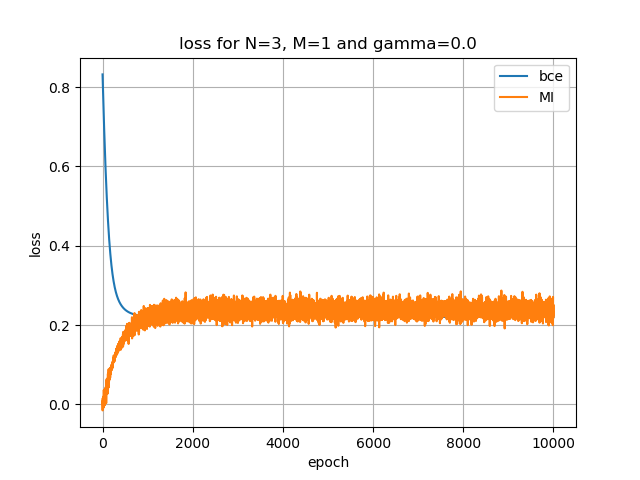
\includegraphics[width=0.8\textwidth]{./gamma_0}
        \caption{\label{fig:gamma_0}BCE loss \& mutual-info}
\end{figure}
%
\begin{figure}
    \centering
        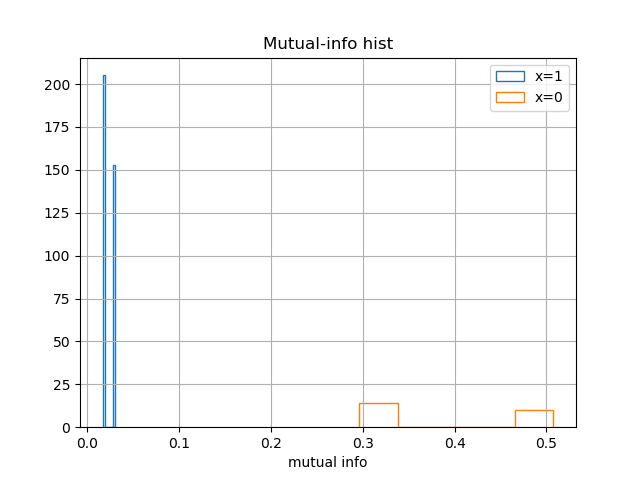
\includegraphics[width=0.8\textwidth]{./mutualInfoHist_gamma_0}
        \caption{\label{fig:mutualInfoHist_gamma_0}mutual-info-hist, $\gamma=0$}
\end{figure}
%
The $\theta$ values the model predicts for $\gamma=0.55$:
%
\begin{center}
 \begin{tabular}{||c | c | c | c | c ||}
 \hline
 Idx & x & t & y & $\theta$ \\ [0.5ex] 
 \hline\hline
 1 & 0 & 1 & 1 & 0.8656 \\ 
 \hline
 2 & 1 & 1 & 0 & 0.1715 \\
 \hline
 3 & 0 & 0 & 0 & 0.1715 \\
 \hline
 4 & 1 & 0 & 1 & 0.4692 \\ [1ex] 
 \hline
\end{tabular}
\end{center}
%
Therefore the ITE is:
%
\begin{equation}
    \begin{split}
        \hat{\tau}_0(x=0) &= \operatorname{E}_{\hat{y}_i^{(l)} \sim p_\phi(\hat{y} \mid t=l,x)}\left[\hat{y}_i^{(1)}-\hat{y}_i^{(0)} \mid x=0 \right]\\
        &= \operatorname{E}_{\hat{y}_i^{(1)} \sim p_\phi(\hat{y} \mid t=1,x=0)}\left[\hat{y}_i^{(1)} \mid x=0 \right] - \operatorname{E}_{\hat{y}_i^{(0)} \sim p_\phi(\hat{y} \mid t=0,x=0)}\left[\hat{y}_i^{(0)} \mid x=0 \right]\\
        &= 0.8656 - 0.1715 = 0.6941\\
        %
        \hat{\tau}_0(x=1) &= \operatorname{E}_{\hat{y}_i^{(l)} \sim p_\phi(\hat{y} \mid t=l,x)}\left[\hat{y}_i^{(1)}-\hat{y}_i^{(0)} \mid x=1 \right]\\
        &= \operatorname{E}_{\hat{y}_i^{(1)} \sim p_\phi(\hat{y} \mid t=1,x=1)}\left[\hat{y}_i^{(1)} \mid x=1 \right] - \operatorname{E}_{\hat{y}_i^{(0)} \sim p_\phi(\hat{y} \mid t=0,x=1)}\left[\hat{y}_i^{(0)} \mid x=1 \right]\\
        &= 0.1715 - 0.4692 = -0.29769    
    \end{split}
\end{equation}
%
While the true ITE is:
\begin{equation}
    \begin{split}
        \tau(x=0) &= 1\\
        \tau(x=1) &= -1
    \end{split}
\end{equation}
%
The ITE percentage error per $x$ value is:
%
\begin{equation}
    \begin{split}
        err(x=0) &= 100\frac{1-0.6941}{1} = 30.58 \%\\
        err(x=1) &= 100\frac{-1-(-0.29769)}{-1} = 70.23\%
    \end{split}
\end{equation}
%
%
\begin{figure}
    \centering
        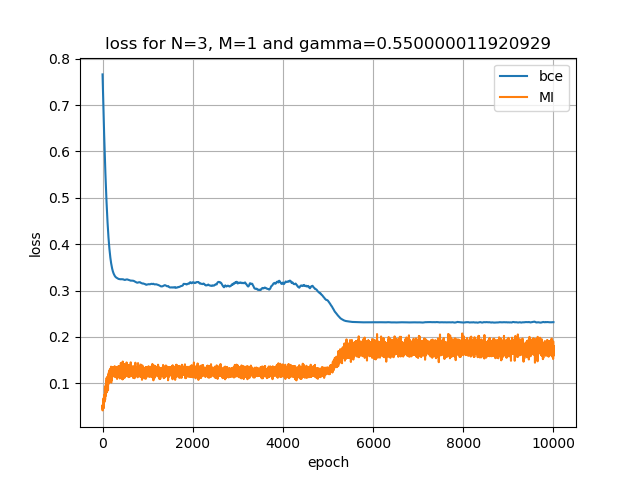
\includegraphics[width=0.8\textwidth]{./mutualInfoHist_gamma_055}
        \caption{\label{fig:mutualInfoHist_gamma_055}BCE loss \& mutual-info}
\end{figure}
%
We repeat all the results in the next two tables and conclude that the model trained with the hybrid BCE-mutual-information loss has improved the ITE for $x=1$ while increasing the error for $x=0$. This is due to the inherent trade-off between the two arguments in the hybrid loss.\\\\ 
Model predictions:
    \begin{center}
     \begin{tabular}{||c | c | c | c | c | c ||}
     \hline
     Idx & x & t & y & $p_\theta(\hat{y}=1 \mid x,t); \gamma=0$ & $p_\theta(\hat{y}=1 \mid x,t); \gamma=0.55$ \\ [0.5ex] 
     \hline\hline
     1 & 0 & 1 & 1 & 0.9499 & 0.8656 \\ 
     \hline
     2 & 1 & 1 & 0 & 0.1391 & 0.1715 \\
     \hline
     3 & 0 & 0 & 0 & 0.1391 & 0.1715 \\
     \hline
     4 & 1 & 0 & 1 & 0.3155 & 0.4692 \\ [1ex] 
     \hline
    \end{tabular}
    \end{center}
ITE errors:
    \begin{center}
     \begin{tabular}{||c | c | c | c | c ||}
     \hline
     x & ITE(x=0) error; $\gamma=0$ & ITE(x=1) error; $\gamma=0.55$ \\ [0.5ex] 
     \hline\hline
     0 & 19\% & 30\% \\ 
     \hline
     1 & 82\% & 70\% \\ [1ex] 
     \hline
    \end{tabular}
    \end{center}
%
%
\section{Theoretical analysis}\label{sec:theo}
We would like to examine the change in log-likelihood and mutual-information due to an update to the learned model. They both will increase if \textbf{a.} the estimated-outcome error decreases and \textbf{b.} the estimated-outcome values become more extreme (Bernoullii distribution tends to 0,1 for a binary outcome). They contradict if the estimated-outcome values become more extreme on expense of an increase in the estimated-outcome error.\\\\
%
We numerically examined the change due an update to the learned-model. Without loss of generality, we focus on an update which changes only the probability of patients with covariates $x_0$ that are not treated - $p(\hat{y} = 1 \mid x_0, t=0)$. For these patients there is a 30\% chance for a positive outcome when not receiving the treatment; Therefore the log-likelihood of the model should peak at $p(\hat{y} = 1 \mid x_0, t=0) = 0.3$. We analyze the change in log-likelihood and mutual information for an infinitesimal update that decreases the probability $p(\hat{y} = 1 \mid x_0, t=0)$ by $0.001$.\\\\
%
In figure \ref{fig:LL_MI} we plotted the log-likelihood and mutual-information values contributed by patients with covariates $x_0$ and different propensity scores. At the lower-left figure we see, as expected, that the log-likelihood value peaks when $p(\hat{y} = 1 \mid x_0, t=0) = 0.3$, yet, the mutual-information value, seen at the lower-right figure, peaks at $p(\hat{y} = 1 \mid x_0, t=0) = 0$. At the upper figures we see that if the leaned-model predicts $p(\hat{y} = 1 \mid x_0, t=0) > 0.3$ than the infinitesimal decrease improves (increases) both the log-likelihood and the mutual information. But, if the leaned-model predicts $p(\hat{y} = 1 \mid x_0, t=0) < 0.3$ than this infinitesimal decrease increases the mutual-information while decreasing the log-likelihood.\\\\
%
\begin{figure}
    \centering
        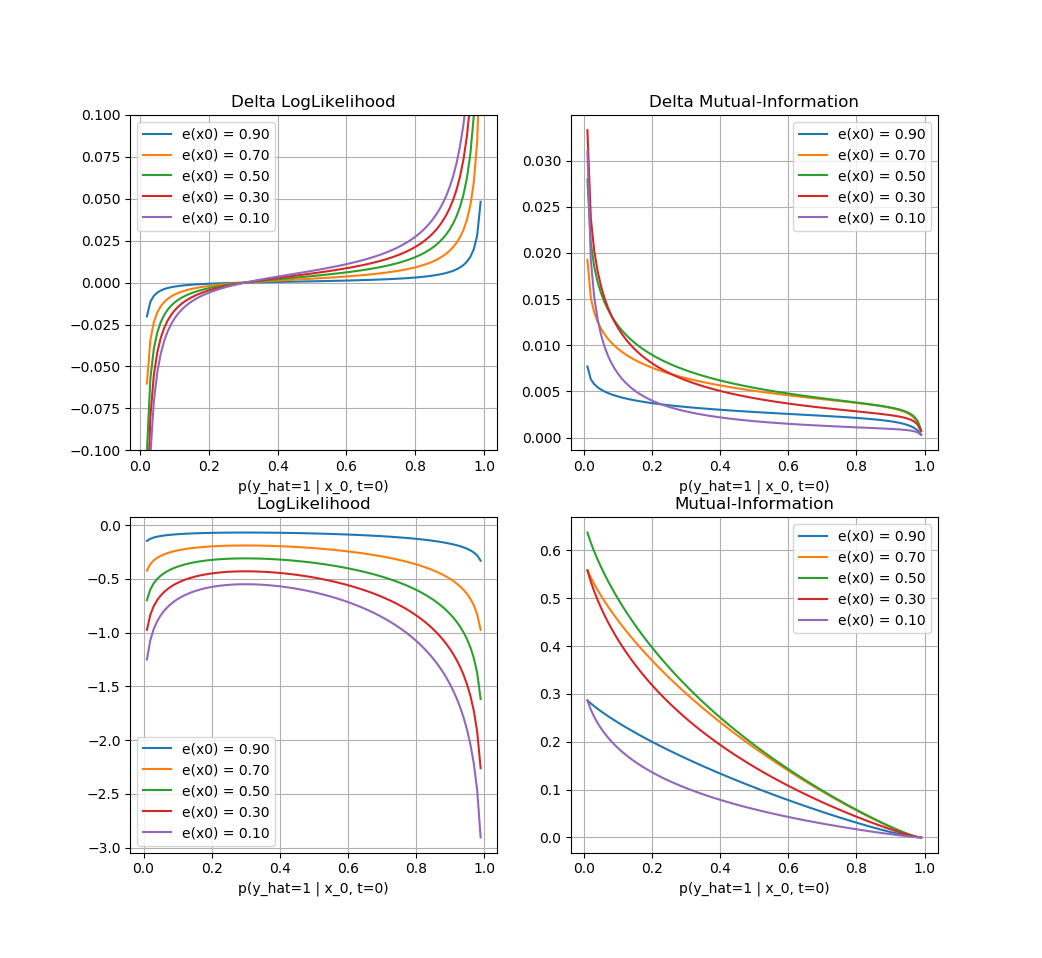
\includegraphics[width=1.0\textwidth]{./LL_MI}
        \caption{\label{fig:LL_MI}Log-likelihood and mutual-information values. In the upper figures the change due to an infinitesimal update to the learned mode; In the lower figures the values of log-likelihood and mutual-information}
\end{figure}
%
The drift away from the correct output distribution of $p(\hat{y} = 1 \mid x_0, t=0)=0.3$ depends on the value of the propensity score of $x_0$ as can be seen in figure \ref{fig:deltaLl_vs_deltaMi}. The learned value of $p(\hat{y} = 1 \mid x_0, t=0)$ will drift away from $0.3$ towards $0$ as long as the increase in mutual-information is higher than the decrease in log-likelihhod. We can see that for patients with low propensity scores the drift is smaller. This is potentially a desired feature of the proposed method. The model that is trained only with respect to log-likelihood is prone to mistake for pairs of (covariates, treatment) that are rare. We focus here on the model-estimation when $t=0$ and note that when $t=0$ is rare (high propensity score) we get a larger region in which the mutual-information is greater than the log-likelihood. This amplifies the attraction towards $p(\hat{y} = 1 \mid x_0, t=0) = 0$ - a desired feature if at the current train-iteration $p(\hat{y} = 1 \mid x_0, t=0) > 0.3$ and undesired if $p(\hat{y} = 1 \mid x_0, t=0) < 0.3$.\\\\
%
\begin{figure}
    \centering
        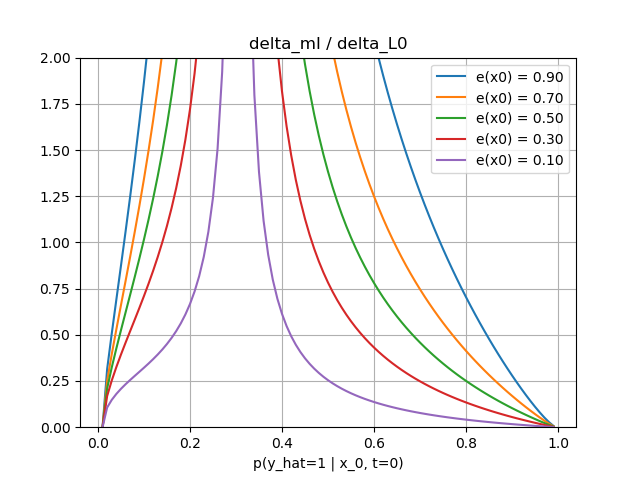
\includegraphics[width=0.8\textwidth]{./deltaLl_vs_deltaMi}
        \caption{\label{fig:deltaLl_vs_deltaMi}Ratio of change in mutual-information to change in log-likelihood due to an update of the learned model for specific covariates. Different propensity scores are displayed.}
\end{figure}
%
We conclude (based just on an 'healthy engineering feel') that the proposed method will have in average a higher outcome estimation error. That is because most estimated outcomes will drift apart from their true values due to the mutual-information loss. Only in specific scenarios and on specific, more rare populations, it might have a lower outcome estimation error. What scenarios exactly do we mean? In many cases the majority of patients respond well to a treatment or are neutral to the treatment. Yet there exists a small fraction of the patients to which the treatment is lethal. We would like to be able to better target these patients even at the cost of a higher false-positive rate. The same concept applies also if some patients have a rare set of covariates and are in great danger pre-treatment assignment. 
%
\section{Twins dataset}\label{sec:twins}
%
The twins dataset is a dataset on twin births, adapted from NBER and manipulated to emulate an observational study. It deals with twins born at a low absolute-weight and considers the treatment as being born with the higher weight. Assuming all covariates for the twins are identical we have here a rare case in which we have both the factual and counterfactual outcomes available. Therefore ITE can be estimated and compared to the true ITE values. See section 4.3 in \cite{NIPS2017_7223} for further details.\\\\
%
We trained\footnote{Code is available at \href{https://github.com/RonTeichner/Benchmarks}{https://github.com/RonTeichner/Benchmarks}} an S-learner \cite{Knzel4156} which is a single learned-model that views the treatment as just another input on top of the covariates. Our model is a simple logistic-regression model - a sigmoid activation function that is applied to an affine transformation of the input. The outcome at the Twins dataset is binary (live or death) and therefore our model outputs the Bernoulli distribution parameter $p(\hat{y}=1 \mid x,t)$. The nominal-train is with respect to the Binary Cross-Entropy (BCE) loss function. We then trained the model with respect to the hybrid BCE - mutual-information loss.\\\\
%
\begin{figure}
    \centering
        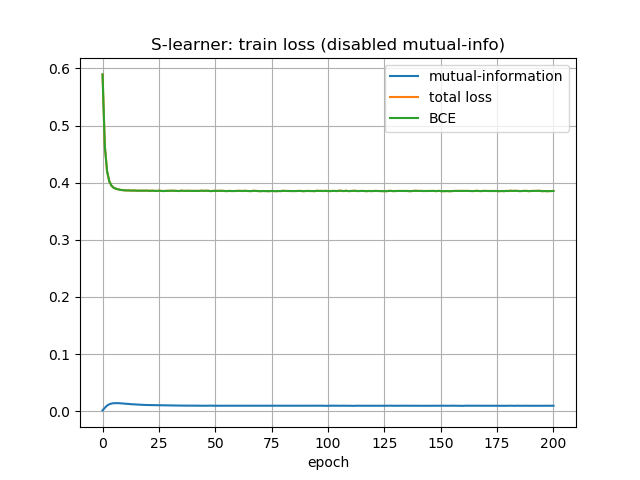
\includegraphics[width=0.8\textwidth]{./train_loss_disableMi}
        \caption{\label{fig:train_loss_disableMi}Train with respect to Binary-Cross-Entropy loss. Mutual-information not included in the loss objective}
\end{figure}
%
\begin{figure}
    \centering
        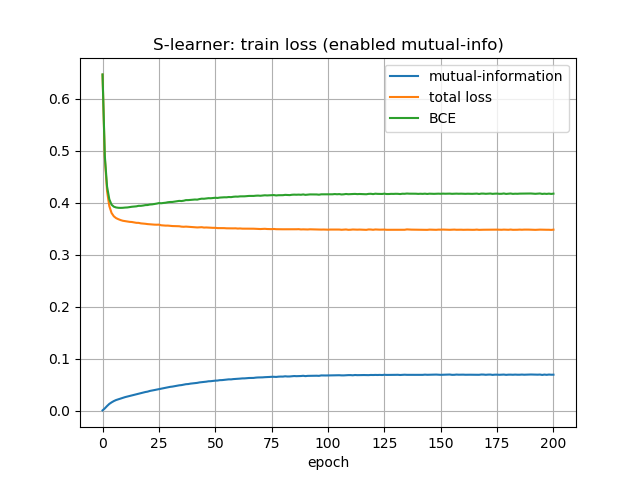
\includegraphics[width=0.8\textwidth]{./train_loss_enableMi}
        \caption{\label{fig:train_loss_enableMi}Train with respect to hybrid Binary-Cross-Entropy & mutual-information loss}
\end{figure}
%
Figures \ref{fig:train_loss_disableMi} and \ref{fig:train_loss_enableMi} depicts the BCE loss, the mutual-information and the total loss when training with respect to BCE loss only (figure \ref{fig:train_loss_disableMi}) and when training with respect to the hybrid loss (figure \ref{fig:train_loss_enableMi}). We can clearly see the result of the losses being in trade-off. While the BCE loss, when training with respect to BCE loss only stabilizes at a value of almost $0.4$, when training with respect to the hybrid loss it stabilizes at a value a-bit higher than $0.4$.\\\\
%
%
\begin{table}[t]
\centering
 \begin{tabular}{||c | c | c | c ||}
 \hline
 Type & BCE-loss & Hybrid-loss & Ground-truth \\ [0.5ex] 
 \hline\hline
 Light twin & 14.97 & 46.35 & 100 \\ 
 \hline
 Heavy twin & 3.9 & 0.65 & 0 \\ [1ex]
 \hline
\end{tabular}
\caption{First group: twins in which the lighter baby does not survive (6.4\% of the dataset). Mortality percentage by hard-decision}
\label{tab:mort1}
\end{table}
%
%
\begin{table}[t]
\centering
 \begin{tabular}{||c | c | c | c ||}
 \hline
 Type & BCE-loss & Hybrid-loss & Ground-truth \\ [0.5ex] 
 \hline\hline
 Light twin & 15.2 & 54.3 & 0 \\ 
 \hline
 Heavy twin & 3 & 0.43 & 100 \\ [1ex]
 \hline
\end{tabular}
\caption{Second group: twins in which the heavier baby does not survive (3.9\% of the dataset). Mortality percentage by hard-decision}
\label{tab:mort2}
\end{table}
%
%
\begin{table}[t]
\centering
 \begin{tabular}{||c | c | c | c | c ||}
 \hline
 Type & BCE-loss & Hybrid-loss & Ground-truth & \% in group \\ [0.5ex] 
 \hline\hline
 Twins survive & 2.6 & 13.67 & 0 & 86\\ 
 \hline
 Twins not survive & 20.57 & 39.4 & 100 & 14\\ [1ex]
 \hline
\end{tabular}
\caption{Third group: twins in which both either survive or not (89.7\% of the dataset). Mortality percentage by hard-decision}
\label{tab:mort3}
\end{table}
%
We analyzed the results for 3 populations. The first consists of twins in which the heavier baby survived and the lighter did not (6.4\% of the dataset); the second consists of twins in which the heavier baby did not survive and the lighter did survive (3.9\% of the dataset); the third group consists of twins that both either survived or not survived (89.7\% of the dataset). For each individual we view the model prediction of mortality probability. We translate the mortality probability into hard-decisions - if it is higher than $0.5$ we say the model predicts mortality. The results are depicted in tables \ref{tab:mort1} - \ref{tab:mort3}. The results on average show a great increase in the estimation outcome error.
%
\begin{itemize}
    \item The largest group are twins in which both twins survive (76.5\% of the dataset). While the model that it trained with respect to BCE loss only predicts that 2.6\% of them will not survive, the model trained on the hybrid loss predicts that 13.6\% of them will not survive. This is an increase in the rate of false-positive.
    \item The second largest group (12.46\%) are twins in which both twins do not survive. In this group we see that the model trained on the hybrid loss predicted that 39.44\% will not survive while the model trained on BCE only predicted that only 20.5\% will not survive. 
    \item The third largest group (6.4\%) are twins in which the lighter twin does not survive and the heavier twin does survive. In this group we see that while the BCE-only model predicts that only 15\% of lighter babies will not survive, the hybrid model predicts that 46.35\% of lighter babies will not survive. This is an improvement, but again we see an increase in false-positive because the hybrid model predicts that 3.9\% of heavier babies will not survive in comparison to 0.6\% according to the BCE only model.
    \item In the last and smallest group (3.99\%) we obtained undesired results - a decrease in the no. of estimated heavy babies that will not survive (hybrid model vs BCE). 
\end{itemize} 
%
\section{Conclusions and future work}\label{sec:goals}
%
We introduced a hybrid loss that on top of a nominal log-likelihood term contains regularization term that encourages high mutual-information between treatment and outcome. We showed on a simple example (Section \ref{sec:example}) that the hybrid loss does amplify the loss for rare inputs in the dataset. This amplification resulted in a decrease of the ITE error for these rare inputs but came at a cost of increasing the ITE error of the majority of inputs. The same phenomena was observed on analysis of results obtained on the Twins dataset (Section \ref{sec:twins}.\\\\
%
We argue that for scenarios in which there is a health risking rare outcome, a rise in the rate of false-positives is acceptable if coupled to an increase in detection performance of the patients in greater danger. 
%
For future work we suggest combining the estimated outcome from two models - one trained with log-likelihood loss only and the other with the hybrid loss. We suggest a combination that weights both the probability of the set of covariates of a patient, $x$ and the propensity score $e(x)$ for combining the two estimations. By identifying the rare patients we could assign them the estimation of the hybrid model which hopefully better fits rare inputs. 
%
%
%\bibliographystyle{Classes/RoboticsBiblio}    % bibliography style
\bibliographystyle{apalike}
\renewcommand{\bibname}{References}           % change default name Bibliography to References
%\addcontentsline{toc}{chapter}{References}    % add References to contents page
\bibliography{References/references}
%
\section{Appendix}\label{sec:appendix}
Mutual information derivation:
\begin{equation}
    \begin{split}
        \operatorname{I}(\hat{y}; t) &= \operatorname{H}(\hat{y}) - \operatorname{H}(\hat{y} \mid t)
    \end{split}
\end{equation}  
%
\begin{equation}
    \begin{split}
        \operatorname{H}(\hat{y}) &= -\operatorname{E}_{\hat{y} \sim p_\theta(\hat{y})}\left[\operatorname{log}p_\theta(\hat{y})\right]\\
        %
        &= -\operatorname{E}_{\hat{y} \sim p_\theta(\hat{y})}\left[\operatorname{log}\sum_{x,t}p_\theta(\hat{y},x,t)\right]\\
        %
        &= -\operatorname{E}_{\hat{y} \sim p_\theta(\hat{y})}\left[\operatorname{log}\sum_{x,t}p_\theta(\hat{y} \mid x,t)p_{data}(x,t)\right]\\
        %
        &= -\operatorname{E}_{x \sim p_{data}(x)}
        \operatorname{E}_{t \sim p_{data}(t \mid x)}
        \operatorname{E}_{\hat{y} \sim p_\theta(\hat{y} \mid x,t)}
        \left[\operatorname{log}\sum_{x,t}p_\theta(\hat{y} \mid x,t)p_{data}(x,t)\right]\\
        %
        &= -\operatorname{E}_{x \sim p_{data}(x)}
        \operatorname{E}_{t \sim p_{data}(t \mid x)}
        \operatorname{E}_{\hat{y} \sim p_\theta(\hat{y} \mid x,t)}
        \left[\operatorname{log}\sum_x p_{data}(x) \sum_{t}p_\theta(\hat{y} \mid x,t)p_{data}(t \mid x)\right]\\
        %
        &= -\operatorname{E}_{x \sim p_{data}(x)}
        \operatorname{E}_{t \sim p_{data}(t \mid x)}
        \operatorname{E}_{\hat{y} \sim p_\theta(\hat{y} \mid x,t)}
        \left[\operatorname{log}\frac{1}{N_B}\sum_x \sum_{t}p_\theta(\hat{y} \mid x,t)p_{data}(t \mid x)\right]\\
        %
        &= -\operatorname{E}_{x \sim p_{data}(x)}
        \operatorname{E}_{t \sim p_{data}(t \mid x)}
        \operatorname{E}_{\hat{y} \sim p_\theta(\hat{y} \mid x,t)}
        \left[\operatorname{log}\frac{1}{N_B}\sum_x e(x)p_\theta(\hat{y} \mid x,1) + (1-e(x))p_\theta(\hat{y} \mid x,0)\right]
    \end{split}
\end{equation}         
%
\\\\
Develop $
        \operatorname{E}_{\hat{y} \sim p_\theta(\hat{y} \mid x,t)}
        \left[\operatorname{log}\frac{1}{N_B}\sum_x e(x)p_\theta(\hat{y} \mid x,1) + (1-e(x))p_\theta(\hat{y} \mid x,0)\right]$:
\begin{equation}
    \begin{split}
        &\operatorname{E}_{\hat{y} \sim p_\theta(\hat{y} \mid x,t)}
        \left[\operatorname{log}\frac{1}{N_B}\sum_x e(x)p_\theta(\hat{y} \mid x,1) (1-e(x))p_\theta(\hat{y} \mid x,0)\right]\\
        %
        &= \theta^{x,t}\left[\operatorname{log}\frac{1}{N_B}\sum_x e(x)\theta^{x,1} + (1-e(x))\theta^{x,0}\right]\\
        &+ (1-\theta^{x,t})\left[\operatorname{log}\frac{1}{N_B}\sum_x e(x)(1-\theta^{x,1}) + (1-e(x))(1-\theta^{x,0})\right]\\
    \end{split}
\end{equation}
%
\\\\
Develop $\operatorname{E}_{t \sim p_{data}(t \mid x)}
        \operatorname{E}_{\hat{y} \sim p_\theta(\hat{y} \mid x,t)}
        \left[\operatorname{log}\frac{1}{N_B}\sum_x e(x)p_\theta(\hat{y} \mid x,1) + (1-e(x))p_\theta(\hat{y} \mid x,0)\right]$:
\begin{equation}
    \begin{split}
        &\operatorname{E}_{t \sim p_{data}(t \mid x)}
        \operatorname{E}_{\hat{y} \sim p_\theta(\hat{y} \mid x,t)}
        \left[\operatorname{log}\frac{1}{N_B}\sum_x e(x)p_\theta(\hat{y} \mid x,1) + (1-e(x))p_\theta(\hat{y} \mid x,0)\right]\\
        %
        &= \operatorname{E}_{t \sim p_{data}(t \mid x)}
        (\theta^{x,t}\left[\operatorname{log}\frac{1}{N_B}\sum_x e(x)\theta^{x,1} + (1-e(x))\theta^{x,0}\right]\\
        &+ (1-\theta^{x,t})\left[\operatorname{log}\frac{1}{N_B}\sum_x e(x)(1-\theta^{x,1}) + (1-e(x))(1-\theta^{x,0})\right])\\
        %
        &= e(x)
        (\theta^{x,1}\left[\operatorname{log}\frac{1}{N_B}\sum_x e(x)\theta^{x,1} + (1-e(x))\theta^{x,0}\right]\\
        &+ (1-\theta^{x,1})\left[\operatorname{log}\frac{1}{N_B}\sum_x e(x)(1-\theta^{x,1}) + (1-e(x))(1-\theta^{x,0})\right])\\
        &+ (1-e(x))(\theta^{x,0}\left[\operatorname{log}\frac{1}{N_B}\sum_x e(x)\theta^{x,1} + (1-e(x))\theta^{x,0}\right]\\
        &+ (1-\theta^{x,0})\left[\operatorname{log}\frac{1}{N_B}\sum_x e(x)(1-\theta^{x,1}) + (1-e(x))(1-\theta^{x,0})\right])\\
        %
        &= \operatorname{log}\frac{1}{N_B} + e(x)
        \left(\theta^{x,1}\operatorname{log}\sum_x \alpha(x)
        + (1-\theta^{x,1})\operatorname{log}\sum_x \beta(x)\right)\\
        &+ (1-e(x))\left(\theta^{x,0}\operatorname{log}\sum_x \alpha(x)
        + (1-\theta^{x,0})\operatorname{log}\sum_x \beta(x)\right)\\
        %
        &= \operatorname{log}\frac{1}{N_B} + e(x)
        \gamma(x,1) + (1-e(x))\gamma(x,0)\\
    \end{split}
\end{equation}
%
We defined:
\begin{equation}
    \begin{split}
        \gamma(x,t) &= \theta^{x,t}\operatorname{log}\sum_x \alpha(x)
        + (1-\theta^{x,t})\operatorname{log}\sum_x \beta(x)\\
        %
        &= \theta^{x,t}\operatorname{log}\sum_x \alpha(x)
        + (1-\theta^{x,t})\operatorname{log}\sum_x (1 - \alpha(x))\\
        %
        \alpha(x) &= e(x)\theta^{x,1} + (1-e(x))\theta^{x,0}\\
        %
        \beta(x) &= e(x)(1-\theta^{x,1}) + (1-e(x))(1-\theta^{x,0}) = 1 - \alpha(x)
    \end{split}
\end{equation}
%
\\\\Develop $\operatorname{E}_{x \sim p_{data}(x)}
        \operatorname{E}_{t \sim p_{data}(t \mid x)}
        \operatorname{E}_{\hat{y} \sim p_\theta(\hat{y} \mid x,t)}
        \left[\operatorname{log}\frac{1}{N_B}\sum_x e(x)p_\theta(\hat{y} \mid x,1) + (1-e(x))p_\theta(\hat{y} \mid x,0)\right]$:
%
\begin{equation}
    \begin{split}
        &\operatorname{E}_{x \sim p_{data}(x)}
        \operatorname{E}_{t \sim p_{data}(t \mid x)}
        \operatorname{E}_{\hat{y} \sim p_\theta(\hat{y} \mid x,t)}
        \left[\operatorname{log}\frac{1}{N_B}\sum_x e(x)p_\theta(\hat{y} \mid x,1) + (1-e(x))p_\theta(\hat{y} \mid x,0)\right]\\
        %
        &= \operatorname{E}_{x \sim p_{data}(x)}\left(\operatorname{log}\frac{1}{N_B} + e(x)\gamma(x,1) + (1-e(x))\gamma(x,0)\right)\\
        %
        &= \frac{1}{N_B}\sum_x \left(\operatorname{log}\frac{1}{N_B} + e(x)\gamma(x,1) + (1-e(x))\gamma(x,0)\right)\\
        %
        &= \operatorname{log}\frac{1}{N_B} + \frac{1}{N_B} \sum_x \left(e(x)\gamma(x,1) + (1-e(x))\gamma(x,0)\right)\\
    \end{split}
\end{equation}
%
To conclude:
\begin{equation}
   \operatorname{H}(\hat{y}) = - \operatorname{log}\frac{1}{N_B} - \frac{1}{N_B} \sum_x \left(e(x)\gamma(x,1) + (1-e(x))\gamma(x,0)\right)
\end{equation}
%
Now develop $\operatorname{H}(\hat{y} \mid t)$:
\begin{equation}
    \begin{split}
        \operatorname{H}(\hat{y} \mid t) &= -\operatorname{E}_{\hat{y},t \sim p_\theta(\hat{y},t)}\left[\operatorname{log}p_\theta(\hat{y} \mid t)\right]\\
        %
        &= -\operatorname{E}_{\hat{y},t \sim p_\theta(\hat{y},t)}\left[\operatorname{log} \sum_x p_\theta(\hat{y},x \mid t)\right]\\
        %
        &= -\operatorname{E}_{\hat{y},t \sim p_\theta(\hat{y},t)}\left[\operatorname{log} \sum_x p_{data}(x) p_\theta(\hat{y} \mid x,t)\right]\\
        %
        &= -\operatorname{E}_{x \sim p_{data}(x)}
        \operatorname{E}_{t \sim p_{data}(t \mid x)}
        \operatorname{E}_{\hat{y} \sim p_\theta(\hat{y} \mid x,t)}
        \left[\operatorname{log} \sum_x p_{data}(x) p_\theta(\hat{y} \mid x,t)\right]\\
    \end{split}
\end{equation}
%
Develop $\operatorname{E}_{\hat{y} \sim p_\theta(\hat{y} \mid x,t)}
        \left[\operatorname{log} \sum_x p_{data}(x) p_\theta(\hat{y} \mid x,t)\right]$:
%
\begin{equation}
    \begin{split}
        &\operatorname{E}_{\hat{y} \sim p_\theta(\hat{y} \mid x,t)}
        \left[\operatorname{log} \sum_x p_{data}(x) p_\theta(\hat{y} \mid x,t)\right]\\
        %
        &= \theta^{x,t}\operatorname{log} \frac{1}{N_B} \sum_x \theta^{x,t} + (1-\theta^{x,t})\operatorname{log} \frac{1}{N_B} \sum_x (1-\theta^{x,t})\\
        %
        &= \operatorname{log} \frac{1}{N_B} + \theta^{x,t}\operatorname{log} \sum_x \theta^{x,t} + (1-\theta^{x,t})\operatorname{log} \sum_x (1-\theta^{x,t})
    \end{split}
\end{equation}
%
Develop $\operatorname{E}_{t \sim p_{data}(t \mid x)}
        \operatorname{E}_{\hat{y} \sim p_\theta(\hat{y} \mid x,t)}
        \left[\operatorname{log} \sum_x p_{data}(x) p_\theta(\hat{y} \mid x,t)\right]$:
%
\begin{equation}
    \begin{split}
        &\operatorname{E}_{t \sim p_{data}(t \mid x)}
        \operatorname{E}_{\hat{y} \sim p_\theta(\hat{y} \mid x,t)}
        \left[\operatorname{log} \sum_x p_{data}(x) p_\theta(\hat{y} \mid x,t)\right]\\
        %
        &= \operatorname{E}_{t \sim p_{data}(t \mid x)} \left(\operatorname{log} \frac{1}{N_B} + \theta^{x,t}\operatorname{log} \sum_x \theta^{x,t} + (1-\theta^{x,t})\operatorname{log} \sum_x (1-\theta^{x,t})\right)\\
        %
        &=e(x)\left( \operatorname{log} \frac{1}{N_B} + \theta^{x,1}\operatorname{log} \sum_x \theta^{x,1} + (1-\theta^{x,1})\operatorname{log} \sum_x (1-\theta^{x,1})\right)\\
        &+ (1-e(x))\left( \operatorname{log} \frac{1}{N_B} + \theta^{x,0}\operatorname{log} \sum_x \theta^{x,0} + (1-\theta^{x,0})\operatorname{log} \sum_x (1-\theta^{x,0})\right)\\
        %
        &=\operatorname{log} \frac{1}{N_B} + e(x)\left(\theta^{x,1}\operatorname{log} \sum_x \theta^{x,1} + (1-\theta^{x,1})\operatorname{log} \sum_x (1-\theta^{x,1})\right)\\
        &+ (1-e(x))\left(\theta^{x,0}\operatorname{log} \sum_x \theta^{x,0} + (1-\theta^{x,0})\operatorname{log} \sum_x (1-\theta^{x,0})\right)\\
        %
        &=\operatorname{log} \frac{1}{N_B} + e(x)a(x,1)
        + (1-e(x))a(x,0)
    \end{split}
\end{equation}
%
We define:
\begin{equation}
    \begin{split}
        a(x,t) = \theta^{x,t}\operatorname{log} \sum_x \theta^{x,t} + (1-\theta^{x,t})\operatorname{log} \sum_x (1-\theta^{x,t})
    \end{split}
\end{equation}
%
Develop $\operatorname{E}_{x \sim p_{data}(x)}
        \operatorname{E}_{t \sim p_{data}(t \mid x)}
        \operatorname{E}_{\hat{y} \sim p_\theta(\hat{y} \mid x,t)}
        \left[\operatorname{log} \sum_x p_{data}(x) p_\theta(\hat{y} \mid x,t)\right]$:
%
\begin{equation}
    \begin{split}
        &\operatorname{E}_{x \sim p_{data}(x)}
        \operatorname{E}_{t \sim p_{data}(t \mid x)}
        \operatorname{E}_{\hat{y} \sim p_\theta(\hat{y} \mid x,t)}
        \left[\operatorname{log} \sum_x p_{data}(x) p_\theta(\hat{y} \mid x,t)\right]\\
        %
        &= \operatorname{E}_{x \sim p_{data}(x)}\left(\operatorname{log} \frac{1}{N_B} + e(x)a(x,1) + (1-e(x))a(x,0)\right)\\
        &= \frac{1}{N_B} \sum_x \left(\operatorname{log} \frac{1}{N_B} + e(x)a(x,1) + (1-e(x))a(x,0)\right)\\
        %
        &= \operatorname{E}_{x \sim p_{data}(x)}\left(\operatorname{log} \frac{1}{N_B} + e(x)a(x,1) + (1-e(x))a(x,0)\right)\\
        %
        &= \operatorname{log} \frac{1}{N_B} + \frac{1}{N_B} \sum_x \left(e(x)a(x,1) + (1-e(x))a(x,0)\right)\\
    \end{split}
\end{equation}
%
To conclude:
\begin{equation}
    \begin{split}
        \operatorname{H}(\hat{y} \mid t) &= -\operatorname{log} \frac{1}{N_B} - \frac{1}{N_B} \sum_x \left(e(x)a(x,1) + (1-e(x))a(x,0)\right)
    \end{split}
\end{equation}
%
So,
\begin{equation}
    \begin{split}
        \operatorname{I}(\hat{y}; t) &= \operatorname{H}(\hat{y}) - \operatorname{H}(\hat{y} \mid t)\\
        &= - \operatorname{log}\frac{1}{N_B} - \frac{1}{N_B} \sum_x \left(e(x)\gamma(x,1) + (1-e(x))\gamma(x,0)\right)\\
        &+\operatorname{log} \frac{1}{N_B} + \frac{1}{N_B} \sum_x \left(e(x)a(x,1) + (1-e(x))a(x,0)\right)\\
        &= \frac{1}{N_B} \sum_x e(x)\left(a(x,1)-\gamma(x,1)\right) + (1-e(x))\left(a(x,0)-\gamma(x,0)\right)
    \end{split}
\end{equation}
%
We defined:
\begin{equation}
    \begin{split}
        a(x,t) &= \theta^{x,t}\operatorname{log} \sum_x \theta^{x,t} + (1-\theta^{x,t})\operatorname{log} \sum_x (1-\theta^{x,t})\\
        %
        \gamma(x,t) &= \theta^{x,t}\operatorname{log}\sum_x \alpha(x)
        + (1-\theta^{x,t})\operatorname{log}\sum_x (1 - \alpha(x))\\
        %
        \alpha(x) &= e(x)\theta^{x,1} + (1-e(x))\theta^{x,0}
    \end{split}
\end{equation}
%
Some results for expectations:
\begin{equation*}
    \begin{split}
        &\operatorname{E}_{x,y,t \sim p(x,y,t)} \left[ f(x,y,t)\right]\\
        &= \int_{x,y,t}p(x,y,t)f(x,y,t)dxdydt\\
        &= \int_{x,y}p(y,x)\left[ \int_t p(t \mid y,x)f(x,y,t)dt\right]dxdy\\
        &= \operatorname{E}_{x,y \sim p(x,y)} \left[\operatorname{E}_{t \sim p(t \mid y,x)}\left[ f(x,y,t)\right] \right]
    \end{split}
\end{equation*}
\\\\
\begin{equation*}
    \begin{split}
        &\operatorname{E}_{t \sim p(t)}\left[f(t)\right]\\
        &= \int_t f(t)p(t)dt\\
        &= \int_t f(t) \left[ \int_x p(t \mid x) p(x) dx \right]dt\\
        &= \int_x p(x)dx \int_t f(t) p(t \mid x) dt\\
        &= \operatorname{E}_{x \sim p(x)} \left[ \operatorname{E}_{t \sim p(t \mid x)} \left[ f(t)\right]\right]
    \end{split}
\end{equation*}
%
\end{document}
